\begin{figure}[t]
\centering
\begin{tabular}{@{}c@{\hspace{4mm}}c@{}}
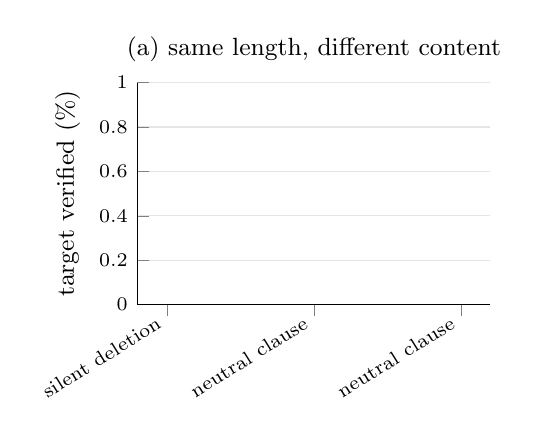
\begin{tikzpicture}
\begin{axis}[
  width=0.50\textwidth, height=4.4cm,
  ybar, bar width=10pt, ymin=0, ymax=100,
  symbolic x coords={silent deletion,neutral clause,irrelevant hedge,positive note,true caveat},
  xtick=data, x tick label style={rotate=32,anchor=east,font=\scriptsize},
  ylabel={target verified (\%)}, ylabel style={font=\small},
  tick label style={font=\scriptsize},
  ymajorgrids, grid style={gray!20}, axis lines*=left,
  title={\small (a) same length, different content}, title style={yshift=-2pt},
]
\addplot+[fill=blue!25,draw=blue!60!black,
  error bars/.cd,y dir=both,y explicit,
  error bar style={line width=0.5pt},error mark options={rotate=90,mark size=2pt}]
  coordinates {\EightArmCoords};
\end{axis}
\end{tikzpicture}
&
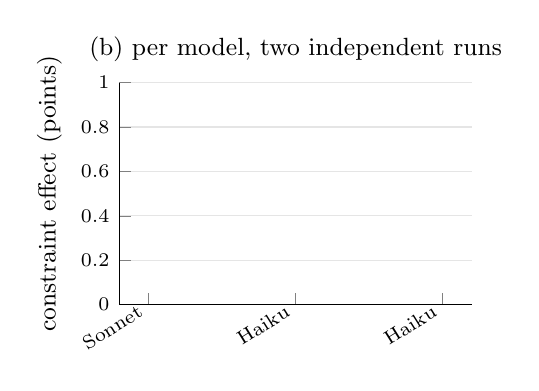
\begin{tikzpicture}
\begin{axis}[
  width=0.50\textwidth, height=4.4cm,
  ymin=-20, ymax=110,
  symbolic x coords={Sonnet,Haiku,Terra,Luna,Sol,Opus},
  xtick=data, x tick label style={rotate=32,anchor=east,font=\scriptsize},
  ylabel={constraint effect (points)}, ylabel style={font=\small},
  tick label style={font=\scriptsize},
  ymajorgrids, grid style={gray!20}, axis lines*=left,
  legend style={font=\scriptsize,at={(0.03,0.97)},anchor=north west,draw=none,fill=none},
  title={\small (b) per model, two independent runs}, title style={yshift=-2pt},
]
\addplot[only marks,mark=*,mark size=2pt,blue!70!black] coordinates {\TenModelPrimaryCoords};
\addlegendentry{primary}
\addplot[only marks,mark=triangle*,mark size=2.6pt,orange!80!black] coordinates {\TenModelReplCoords};
\addlegendentry{replication}
\draw[dashed,gray] (axis cs:Sonnet,\TenPooledLine) -- (axis cs:Opus,\TenPooledLine);
\draw[gray!60] (axis cs:Sonnet,0) -- (axis cs:Opus,0);
\end{axis}
\end{tikzpicture}
\end{tabular}
\caption{\textbf{(a)} Experiment 8, \EightN{} episodes. Four arms append a
clause of \EightAppendMin--\EightAppendMax{} characters; \emph{silent
deletion} appends none. An irrelevant hedge sits on the neutral clause
(\EightHedgeVsPadded{} points, $p = \EightHedgeVsPaddedP$): the earlier hedging
interpretation does not survive its own length control. The true caveat is
\EightCaveatVsPadded{} points below that neutral clause. Wilson 95\% intervals.
\textbf{(b)} Experiment 10 constraint effect per model, primary run and
pre-registered replication, over \TenContrastN{} episodes; dashed line the
pooled estimate (\TenPooled), solid line zero. Positive in \TenPosPrimary{} of
\TenModels{} models primary and \TenPosRepl{} of \TenModels{} replicated;
\TenFlippedModel{} is the only sign difference between runs and the least
stable model under repeated identical prompts.}
\label{fig:resolved}
\end{figure}
